\documentclass[10pt,UTF8]{article}

\usepackage{geometry}

\usepackage{ctex}

\geometry{a4paper,scale=0.9}
\ctexset{today=old}

\usepackage[bookmarksnumbered=true]{hyperref}  % 生成大纲


\usepackage{times}  % 设置正文字体为 Adobe Times Roman

\usepackage{amsmath}
\usepackage{amssymb}
\usepackage{mathtools}

\usepackage{physics}


%%%%%%%%%%%%%%%%%%%%%%%% tcolorbox %%%%%%%%%%%%%%%%%%%%%%%%%%
\usepackage[most]{tcolorbox}

\newenvironment{definition box}
{\begin{tcolorbox}[colback=blue!5!white,colframe=blue!75!black,parbox=false,before upper=\par,before lower=\par]}
{\end{tcolorbox}}

%%%%%%%%%%%%%%%%%%%%%%%%%%%%%%%%%%%%%%%%%%%%%%%%%%%%%%%%%%%%
            
%%%%%%%%%%%%%%%%%%%%% amsthm %%%%%%%%%%%%%%%%
\usepackage{amsthm}

\theoremstyle{definition}
\newtheorem*{definition inner}{Definition}
\newenvironment{definition}[1][]
{\begin{definition box}\begin{definition inner}[#1]\hfill\par}
{\end{definition inner}\end{definition box}}

\theoremstyle{remark}
\newtheorem*{remark}{\textit{Remark}}
%%%%%%%%%%%%%%%%%%%%%%%%%%%%%%%%%%%%%%%%%%%%%%

\newcommand{\mycases}[2][0.8]{
    \left\{\vphantom{\scalebox{#1}{
        $\begin{matrix}#2\end{matrix}$
    }}\right.\!\!\!\!
    \begin{array}{l@{\quad}l}#2\end{array}
}

\newcommand{\ju}{\mathrm{j}}  % 虚数单位
\newcommand{\e}{\mathrm{e}{\mkern 1 mu}}

\newcommand{\Ev}[1]{\mathcal{E}\textit{v}\!\left\{#1\right\}}
\newcommand{\Od}[1]{\mathcal{O}\textit{d}\!\left\{#1\right\}}


\begin{document}


\section{Signals and Systems}


\paragraph{Signals}
A signal is a function of one or more \emph{independent} variables.

\begin{itemize}
    \item Continuous-time signals: $x(t)$, where $t$ is a continuous variable.
    \item Discrete-time signals: $x[n]$, where $n$ is a discrete variable.
\end{itemize}

\paragraph{Systems}
A system is a process that transforms signals.



\section{Energy and Average Power}

For a signal $x(t)$ or $x[n]$ (usually takes on \emph{complex values}),
the energy and average power are defined as:

\noindent
\begin{minipage}[t]{0.45\textwidth}
    \subsection{Discrete-Time}
    \begin{definition}[Energy]
        \subparagraph{}Over a time interval $[n_1, n_2]$:
        \[
            \sum_{n=n_1}^{n_2} \abs{x[n]}^2
        \]
        \subparagraph{}Over an infinite time interval:
        \[
            E_{\infty} := \lim_{N\to\infty} \sum_{n=-N}^N \abs{x[n]}^2
            = \sum_{n=-\infty}^{\infty} \abs{x[n]}^2
        \]
    \end{definition}
    \begin{definition}[Average Power]
        \subparagraph{}Over a time interval $[n_1, n_2]$:
        \[
            \frac{1}{n_2 - n_1 + 1} \sum_{n=n_1}^{n_2} \abs{x[n]}^2
        \]
        \subparagraph{}Over an infinite time interval:
        \[
            P_{\infty} := \lim_{N\to\infty} \frac{1}{2 N+1} \sum_{n=-N}^N \abs{x[n]}^2
        \]
    \end{definition}
\end{minipage}\hfill
\begin{minipage}[t]{0.45\textwidth}
    \subsection{Continuous-Time}
    \begin{definition}[Energy]
        \subparagraph{}Over a time interval $[t_1, t_2]$:
        \[
            \int_{t_1}^{t_2} \abs{x(t)}^2 \dd{t}
        \]
        \subparagraph{}Over an infinite time interval:
        \[
            E_{\infty} := \lim_{T\to\infty} \int_{-T}^T \abs{x(t)}^2 \dd{t}
            = \int_{-\infty}^{\infty} \abs{x(t)}^2 \dd{t}
        \]
    \end{definition}
    \begin{definition}[Average Power]
        \subparagraph{}Over a time interval $[t_1, t_2]$:
        \[
            \frac{1}{t_2 - t_1} \int_{t_1}^{t_2} \abs{x(t)}^2 \dd{t}
        \]
        \subparagraph{}Over an infinite time interval:
        \[
            P_{\infty} := \lim_{T\to\infty} \frac{1}{2 T} \int_{-T}^T \abs{x(t)}^2 \dd{t}
        \]
    \end{definition}
\end{minipage}



\subsection{Cases of Energy and Average Power}
\begin{center}
\begin{tabular}
    { c @{\qquad}|@{\qquad\qquad} c @{\qquad\qquad\qquad} c @{\qquad\qquad\qquad} c }
     & $E_{\infty}$ & $P_{\infty}$ & Remark \\\hline\\
    Case 1 & $0$ & $0$ & iff the signal is always zero. \\\\
    Case 2 & finite & $0$ \\\\
    Case 3 & $\infty$ & finite \\\\
    Case 4 & $\infty$ & $\infty$    
\end{tabular}
\end{center}



\section{Transformations of the Independent Variable}

\begin{itemize}
    \item Time Shift
    \item Time Reversal
    \item Time Scaling
\end{itemize}


\section{Periodic and Aperiodic Signals}

If a signal $x(t)$ or $x[n]$ is periodic with period $T$ or $N$,
where $T$ or $N$ is positive, then
\begin{equation*}
    x(t+T) = x(t) \qor x[n+N] = x[n]
\end{equation*}

\textbf{Fundamental Period} $T_0$ or $N_0$:
the smallest positive value of $T$ or $N$.


\section{Even and Odd Signals}

\begin{definition}[Even-Odd Decomposition]
    \begin{align*}
        \Ev{x[n]} &:= \frac{1}{2} \Big[x[n] + x[-n]\Big] &
        \Ev{x(t)} &:= \frac{1}{2} \Big[x(t) + x(-t)\Big] \\
        \Od{x[n]} &:= \frac{1}{2} \Big[x[n] - x[-n]\Big] &
        \Od{x(t)} &:= \frac{1}{2} \Big[x(t) - x(-t)\Big]
    \end{align*}
\end{definition}

Then we have:
\begin{align*}
    x[n] &= \Ev{x[n]} + \Od{x[n]} &
    x(t) &= \Ev{x(t)} + \Od{x(t)} 
\end{align*}


\section{Exponential and Sinusoidal Signals}

\subsection{General Complex Exponential Signals}

Let $C = \abs{C}\e^{\ju\theta}$ and $a = r + \ju\omega_0$.
\begin{equation*}
    x(t) = C \e^{a t} = 
    \abs{C} \e^{r t}\Big[\cos(\omega_0 t+\theta)+\ju\sin(\omega_0 t+\theta)\Big]
\end{equation*}

Let $C = \abs{C}\e^{\ju\theta}$ and $\alpha = \abs{\alpha}\e^{\ju\omega_0}$.
\begin{equation*}
    x[n] = C \alpha^n = 
    \abs{C}\abs{\alpha}^n\Big[\cos(\omega_0 n+\theta)+\ju\sin(\omega_0 n+\theta)\Big]
\end{equation*}

\subsection{periodicity}

\subsubsection{Continuous-Time}

\begin{itemize}
    \item A \emph{complex exponential signal} $x(t) = C \e^{a t}$,
    where $a = r + \ju\omega_0$, is periodic \textbf{iff} $r = 0$.
    \item A \emph{sinusoidal signal} $x(t) = A\sin(\omega_0 t+\phi)$
    is \textbf{always} periodic.
    \item When $\omega_0 \ne 0$,
    the \emph{fundamental period} for both of them
    is $T_0=\dfrac{2\pi}{\abs{\omega_0}}$.
\end{itemize}

\begin{remark}
    Actually, the sinusoidal signal is just a special case of the complex exponential signal,
    where $r = 0$, thus it must be periodic.
\end{remark}

\subsubsection{Discrete-Time}

\begin{itemize}
    \item A \emph{complex exponential signal} $x[n] = C \alpha^n$,
    where $\alpha = \abs{\alpha}\e^{\ju\omega_0}$, is periodic \textbf{iff}
    $\abs{\alpha} = 1$ and $\abs{\omega_0} = \dfrac{2\pi m}{N}$
    for some $N,m\in\mathbb{N}$
    (i.e., $\omega_0$ must be a rational multiple of $\pi$).
    \item A \emph{sinusoidal signal} $x[n] = A\sin(\omega_0 n+\phi)$
    is periodic \textbf{iff} $\abs{\omega_0} = \dfrac{2\pi m}{N}$
    for some $N,m\in\mathbb{N}$
    (i.e., $\omega_0$ must be a rational multiple of $\pi$).
    \item When $\omega_0 \ne 0$,
    the \emph{fundamental period} for both of them
    is $N_0=\dfrac{2\pi m}{\abs{\omega_0}}$,
    where $m$ is the least integer such that $N_0\in\mathbb{Z}_+$.
\end{itemize}

\begin{remark}
    The sinusoidal signal is just a special case of the complex exponential signal,
    where $\abs{\alpha} = 1$.
\end{remark}

\section{Unit Step and Unit Impulse Functions}

\subsection{Discrete-Time}

\noindent
\begin{minipage}[t]{.45\textwidth}
    \begin{definition}[Unit Step Function]
        \[
            u[n] := \mycases{
                1, & n \geqslant 0 \\
                0, & n < 0
            }
        \]
        $u[n]$ is the \emph{running sum} of $\delta[n]$, i.e.,
        \[
            u[n] = \sum_{k=-\infty}^n \delta[k]
        \]
    \end{definition}
\end{minipage}\hfill
\begin{minipage}[t]{.45\textwidth}
    \begin{definition}[Unit Impulse Function]
        \[
            \delta[n] := \mycases{
                0, & n \ne 0 \\
                1, & n = 0
            }
        \]
        $\delta[n]$ is the \emph{first difference} of $u[n]$, i.e.,
        \[
            \delta[n] = u[n] - u[n-1]
        \]
    \end{definition}
\end{minipage}

\subsection{Continuous-Time}

First we define:
\[
u_{_\Delta}(t) := \mycases{
    0, & t < 0 \\
    \frac{t}{\Delta}, & 0 \leqslant t \leqslant \Delta \\
    1, & t > \Delta
}
\qquad\qquad\qquad\qquad\qquad\qquad
\delta_{_\Delta}(t) := \dv{u_{_\Delta}(t)}{t}
\]

Then we can define:

\noindent
\begin{minipage}[t]{.45\textwidth}
\begin{definition}[Unit Step Function]
    \[
        u(t) := \mycases{
            1, & t > 0 \\
            0, & t < 0
        }
    \]
\end{definition}
    $u(t)$ is the \emph{running integral} of $\delta(t)$, i.e.,
    \[
        u(t) = \int_{-\infty}^t \delta(\tau) \dd\tau
    \]
\end{minipage}\hfill
\begin{minipage}[t]{.45\textwidth}
    \begin{definition}[Unit Impulse Function]
        \[
            \delta(t) := \lim_{\Delta\to 0^+}\delta_{_\Delta}(t)
        \]
    \end{definition}
    $\delta(t)$ is the \emph{first derivative} of $u(t)$, i.e.,
    \[
        \delta(t) = \dv{u(t)}{t}
    \]
\end{minipage}

\subsection{Properties}

\begin{gather*}
    f(t)\delta(t-t_0) = f(t_0)\delta(t-t_0) \qquad\qquad
\int_{-\infty}^{t}f(\tau)\delta(\tau)\dd{\tau} = f(0) u(t)
\shortintertext{
Note that
the Fundamental Theorems of Calculus
do not hold as
$f(\tau)\delta(\tau)$
is not continuous.
}
\int_{a}^{b}f(\tau)\delta(\tau)\dd{\tau} =
f(0) \Big[u(-a) u(b)-u(a)u(-b)\Big] \\
\int_{a}^{b}f(\tau)u(\tau)\dd{\tau} = \int_{u(a)a}^{u(b)b}f(\tau)\dd{\tau} \\
\end{gather*}

\section{Interconnections of Systems}

We can use \emph{block diagrams} to represent the interconnections of systems.

\subsection{Series (Cascade) Interconnection}

A \emph{series} or \emph{cascade} \emph{interconnection} of two systems is shown in the following block diagram:
\begin{center}
    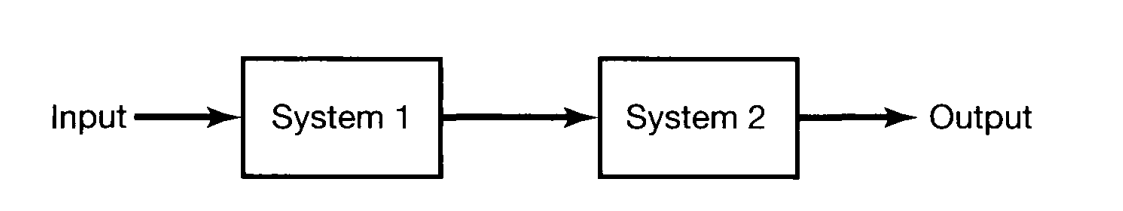
\includegraphics[width=0.6\textwidth]{assets/A Series Interconnection.png}
\end{center}

\subsection{Parallel Interconnection}
\begin{center}
    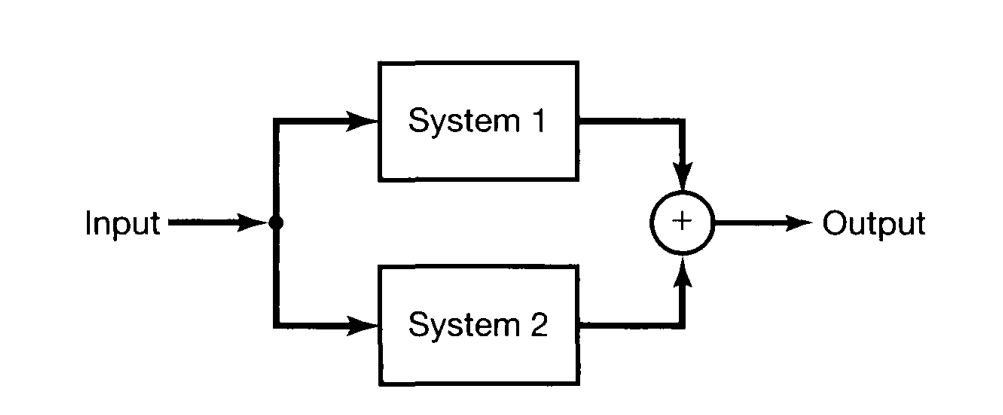
\includegraphics[width=0.5\textwidth]{assets/A Parallel Interconnection.png}
\end{center}

\subsection{Feedback Interconnection}
\begin{center}
    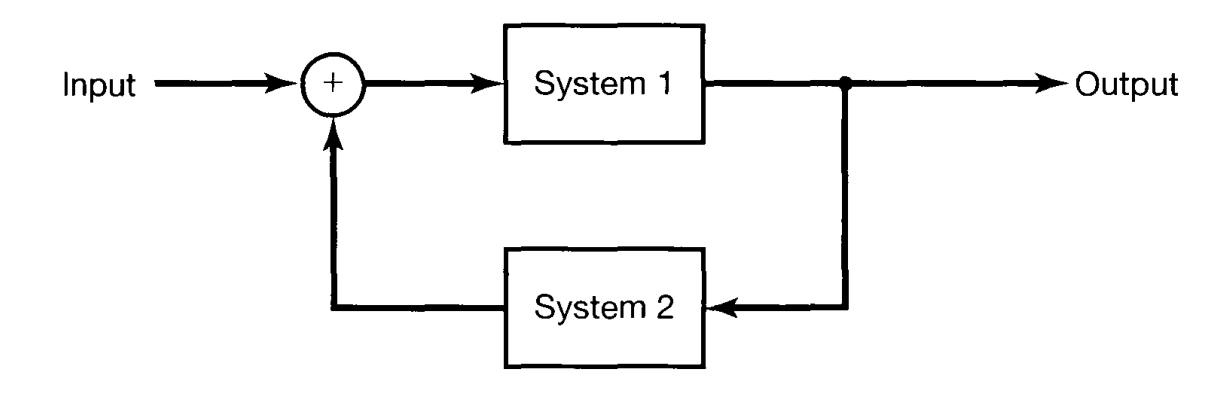
\includegraphics[width=0.5\textwidth]{assets/A Feedback Interconnection.png}
\end{center}



\section{Basic System Properties}

\subsection{Memory}

\begin{definition}[Memoryless]
    A system is said to be \emph{memoryless}
    if its output for each value of the independent variable
    at a given time is dependent \textbf{only on the input at that same time}. 
\end{definition}

\subsection{lnvertibility}

\begin{definition}[Invertible]
    A system is said to be \emph{invertible}
    if distinct inputs lead to distinct outputs.
\end{definition}

\subsection{Causality}

\begin{definition}[Causal]
    A system is \emph{causal}
    if the output at any time depends only on values of the input at the
    present time and in the past.
\end{definition}

Such a system is often referred to as being \emph{nonanticipative},
as the system output does not anticipate future values of the input.

\subsection{Stability}

\begin{definition}[Stable]
    A system is \emph{stable} if
    \textbf{b}ounded \textbf{i}nput gives \textbf{b}ounded \textbf{o}utput
    (BIBO).
\end{definition}

\subsection{Time lnvariance}

\begin{definition}[Time-Invariant]
    A system is \emph{time-invariant} if a time shift in the input only
    causes a time shift in the output.
    Otherwise, it is \emph{time-variant}.
\end{definition}

A system $S$ is \emph{time-invariant} iff it satisfies:
\begin{gather*}
    x(t) \xlongrightarrow{S} y(t) \quad \implies \quad
    x(t+\tau) \xlongrightarrow{S} y(t+\tau) \\
    \shortintertext{or}
    x[n] \xlongrightarrow{S} y[n] \quad \implies \quad
    x[n+n_0] \xlongrightarrow{S} y[n+n_0]
\end{gather*}

\subsection{Linearity}

\begin{definition}[Linear]
    A system $S$ is \emph{linear} if it satisfies the following two properties:
    \begin{itemize}
        \item \emph{Additivity}: 
            $x_1(t) + x_2(t) \xlongrightarrow{S} y_1(t) + y_2(t)$
        \item \emph{Scaling} or \emph{Homogeneity}:
            $a\cdot x(t) \xlongrightarrow{S} \cdot y(t)$
    \end{itemize}
\end{definition}

If linear, then \textbf{z}ero \textbf{i}nput gives \textbf{z}ero \textbf{o}utput (ZIZO).


\subsection{Linear Time-Invariant (LTI) Systems}

Systems that are both linear and time-invariant.




\end{document}
